\documentclass[a4paper,12pt]{article}
\usepackage{mathrsfs}
\usepackage{geometry}
\usepackage{tcolorbox}
\geometry{a4paper,left=2.5cm,right=2cm,top=2cm,bottom=2cm}

\begin{document}
	\section{Purpose of this DAQ ?}
	I wrote this DAQ in the hope for it to become the (prototype of)
	standard DAQ used by IMP. As far as I learned, by the time this DAQ was
	written, no `standard' DAQ existed in IMP and nobody was working on
	this, even (probably) nobody was thinking about such a thing. This is,
	in my humble opinion, one major thing that we were behind others (e.g.
	GSI, NSCL/FRIB). However, to really develop a universal DAQ applicable
	to many experiments, we may need a whole group to do that. I cannot do
	that on my own. So in this version of DAQ, I kept many things as simple
	as possible and many things remained unoptimized. The bottom line was to
	make sure that it works and can be easily used by others. How easy could
	it be ? Well, in most cases, one should be able to set it up by just
	clicking mouse and fill in some parameters (like module base addresses)
	without any coding (except for the online analysis part). To that end,
	one has to use only the modules predefined in this DAQ, unsupported
	modules won't work properly (in fact, they won't work at all). What if
	one needs to use an unsupported module? There are three ways to work it
	around: i) find an alternative module; ii) contact me to include your
	module (gaobsh@impcas.ac.cn); iii) do it yourself, you should be able to
	include your module easily since special care was taken to accomplish
	that.

	Special care was also taken to make sure the DAQ can be
	upgraded to be used in more complicated experiments with minimal
	modifications (extensibility). That means although the current version
	is kept as simple as possible, it can be easily extended to a more
	complex version. Why not design it to be a complex DAQ in the first
	place? Well, there are many reasons. First, I don't have time to do
	that. Second, more complicated system required high learning curve,
	which may hindrance people from using it. Third, as far as I can see,
	there is still no (or very little) such demands from the IMP.

	Part of the DAQ designment is inspired by the NSCL DAQ.

	\section{Overview of the DAQ}
	\begin{figure}
		\begin{center}
			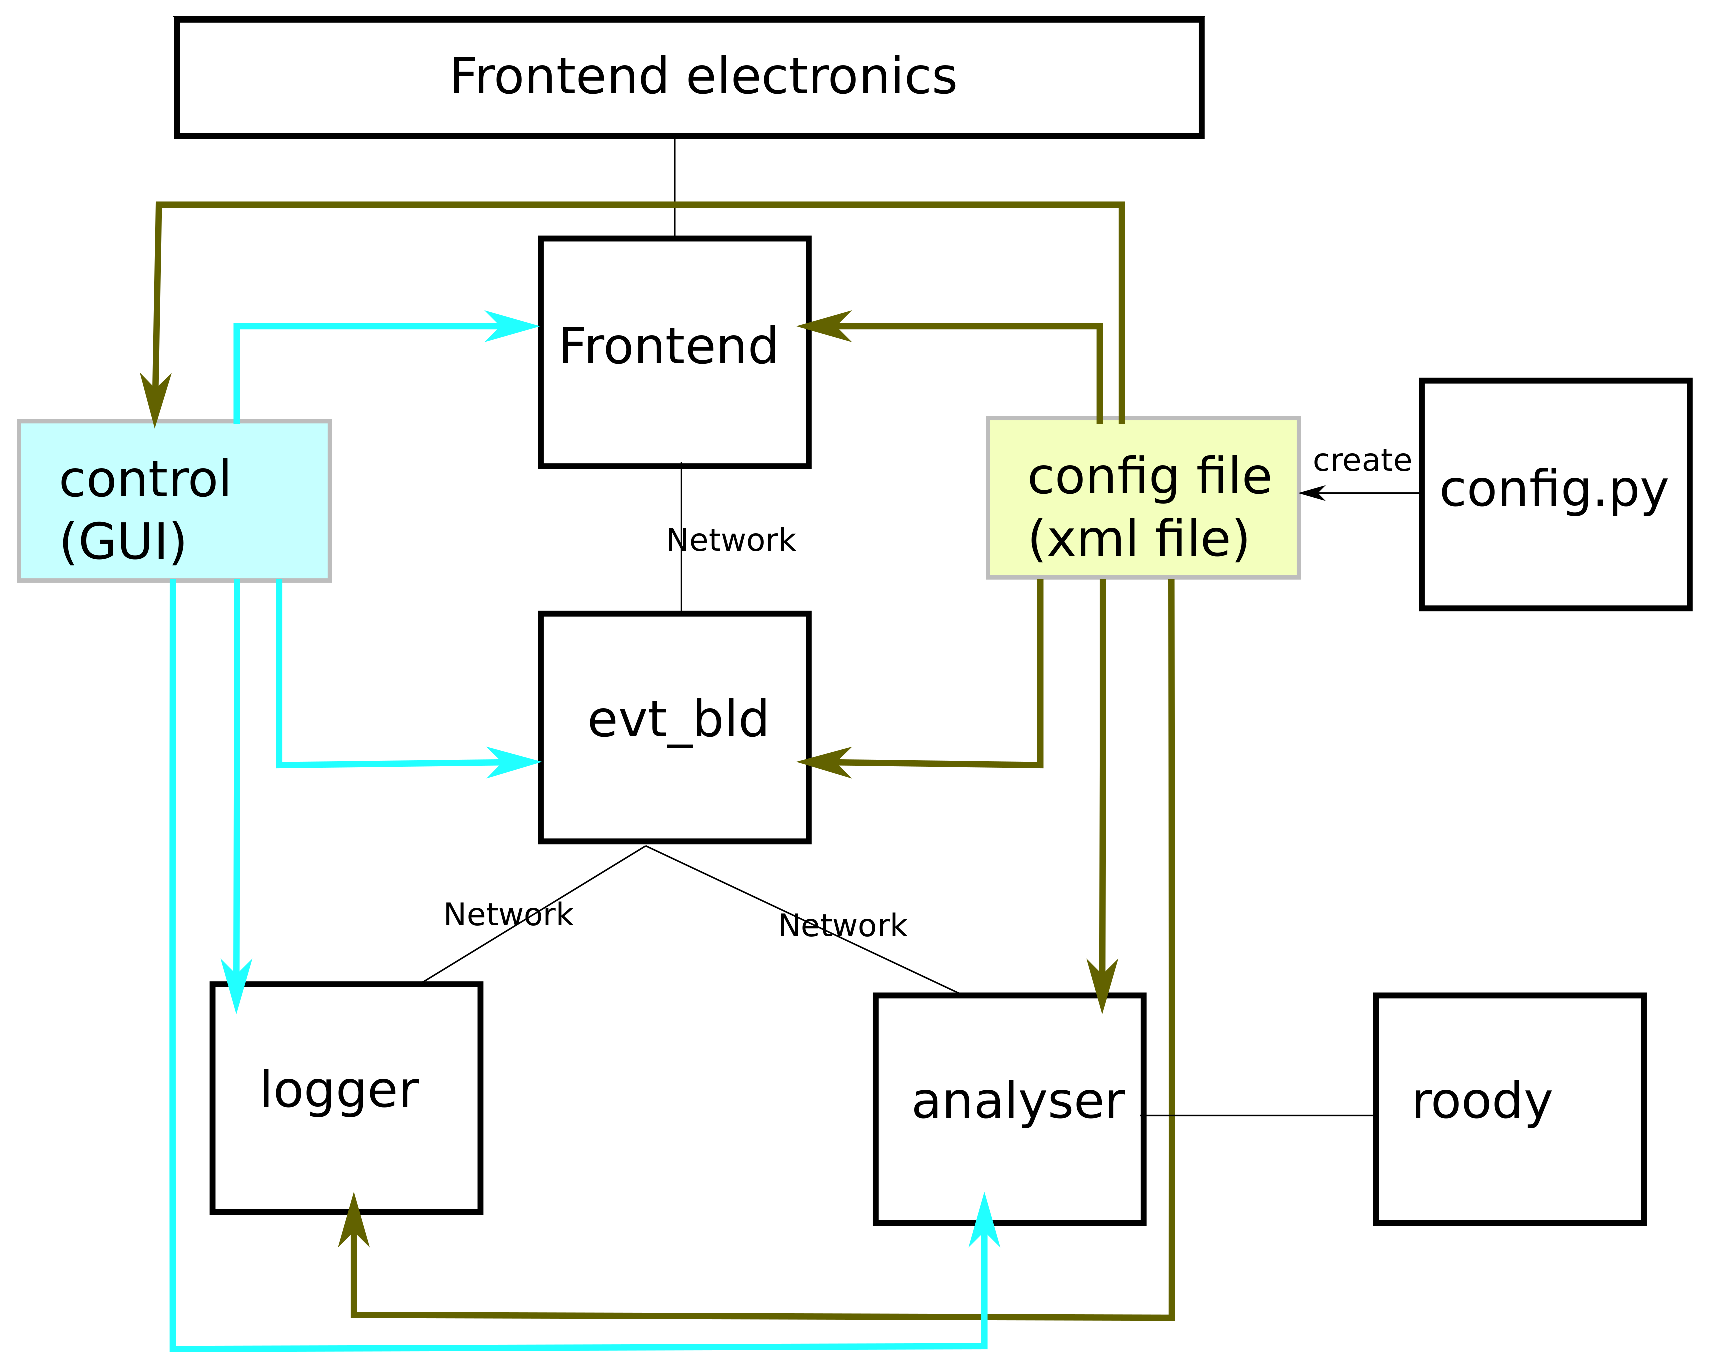
\includegraphics[width=.4\textwidth]{figs/daq_scheme.eps}
			\caption{\label{fig01}Components of the DAQ }
		\end{center}
	\end{figure}
	This DAQ consists of the following parts, see Fig. \ref{fig01}:
	\begin{itemize}
		\item config.py. This is a GUI program (python script) to help user
			create the configuration file used by the DAQ.
		\item frontend. This is the part that communicates with the
			electronics (e.g. VME modules).
		\item evt\_bld. This is the event builder. It grabs data from the
			frontend and build a complete event based on timestamps of the
			fragments readout by frontend.
		\item logger. This program takes data from evt\_bld and records it
			in hard drives.
		\item analyser. This program also takes data from evt\_bld, it
			analysis the events and makes histograms instead of recording
			them.
	\end{itemize}
	The communications between different programs is done via sockets. I
	chose sockets instead of shared memory based on the following
	considerations:
	 i) Different programs do NOT have to run in the same computer. This
	 makes the DAQ more extendable. It also avoids the analyser slowing down
	 the DAQ when it takes too much CPU time.
	 ii) The synchronisation becomes easier because mutex or semaphores are
	 not needed in between programs (although they may still be needed
	 inside a program containing multi threads). Sockets are also easier to
	 handle (as far as I'm concerned).
	 iii) The sockets are of cause slower than shared memory, however, it
	 should not be a problem in most cases.

	 In principle only the frontend and analyser may need the configuration,
	 however, I designed it such that all components read in the
	 configuration file at startup in case it may be needed in the future.
	\begin{figure}
		\begin{center}
			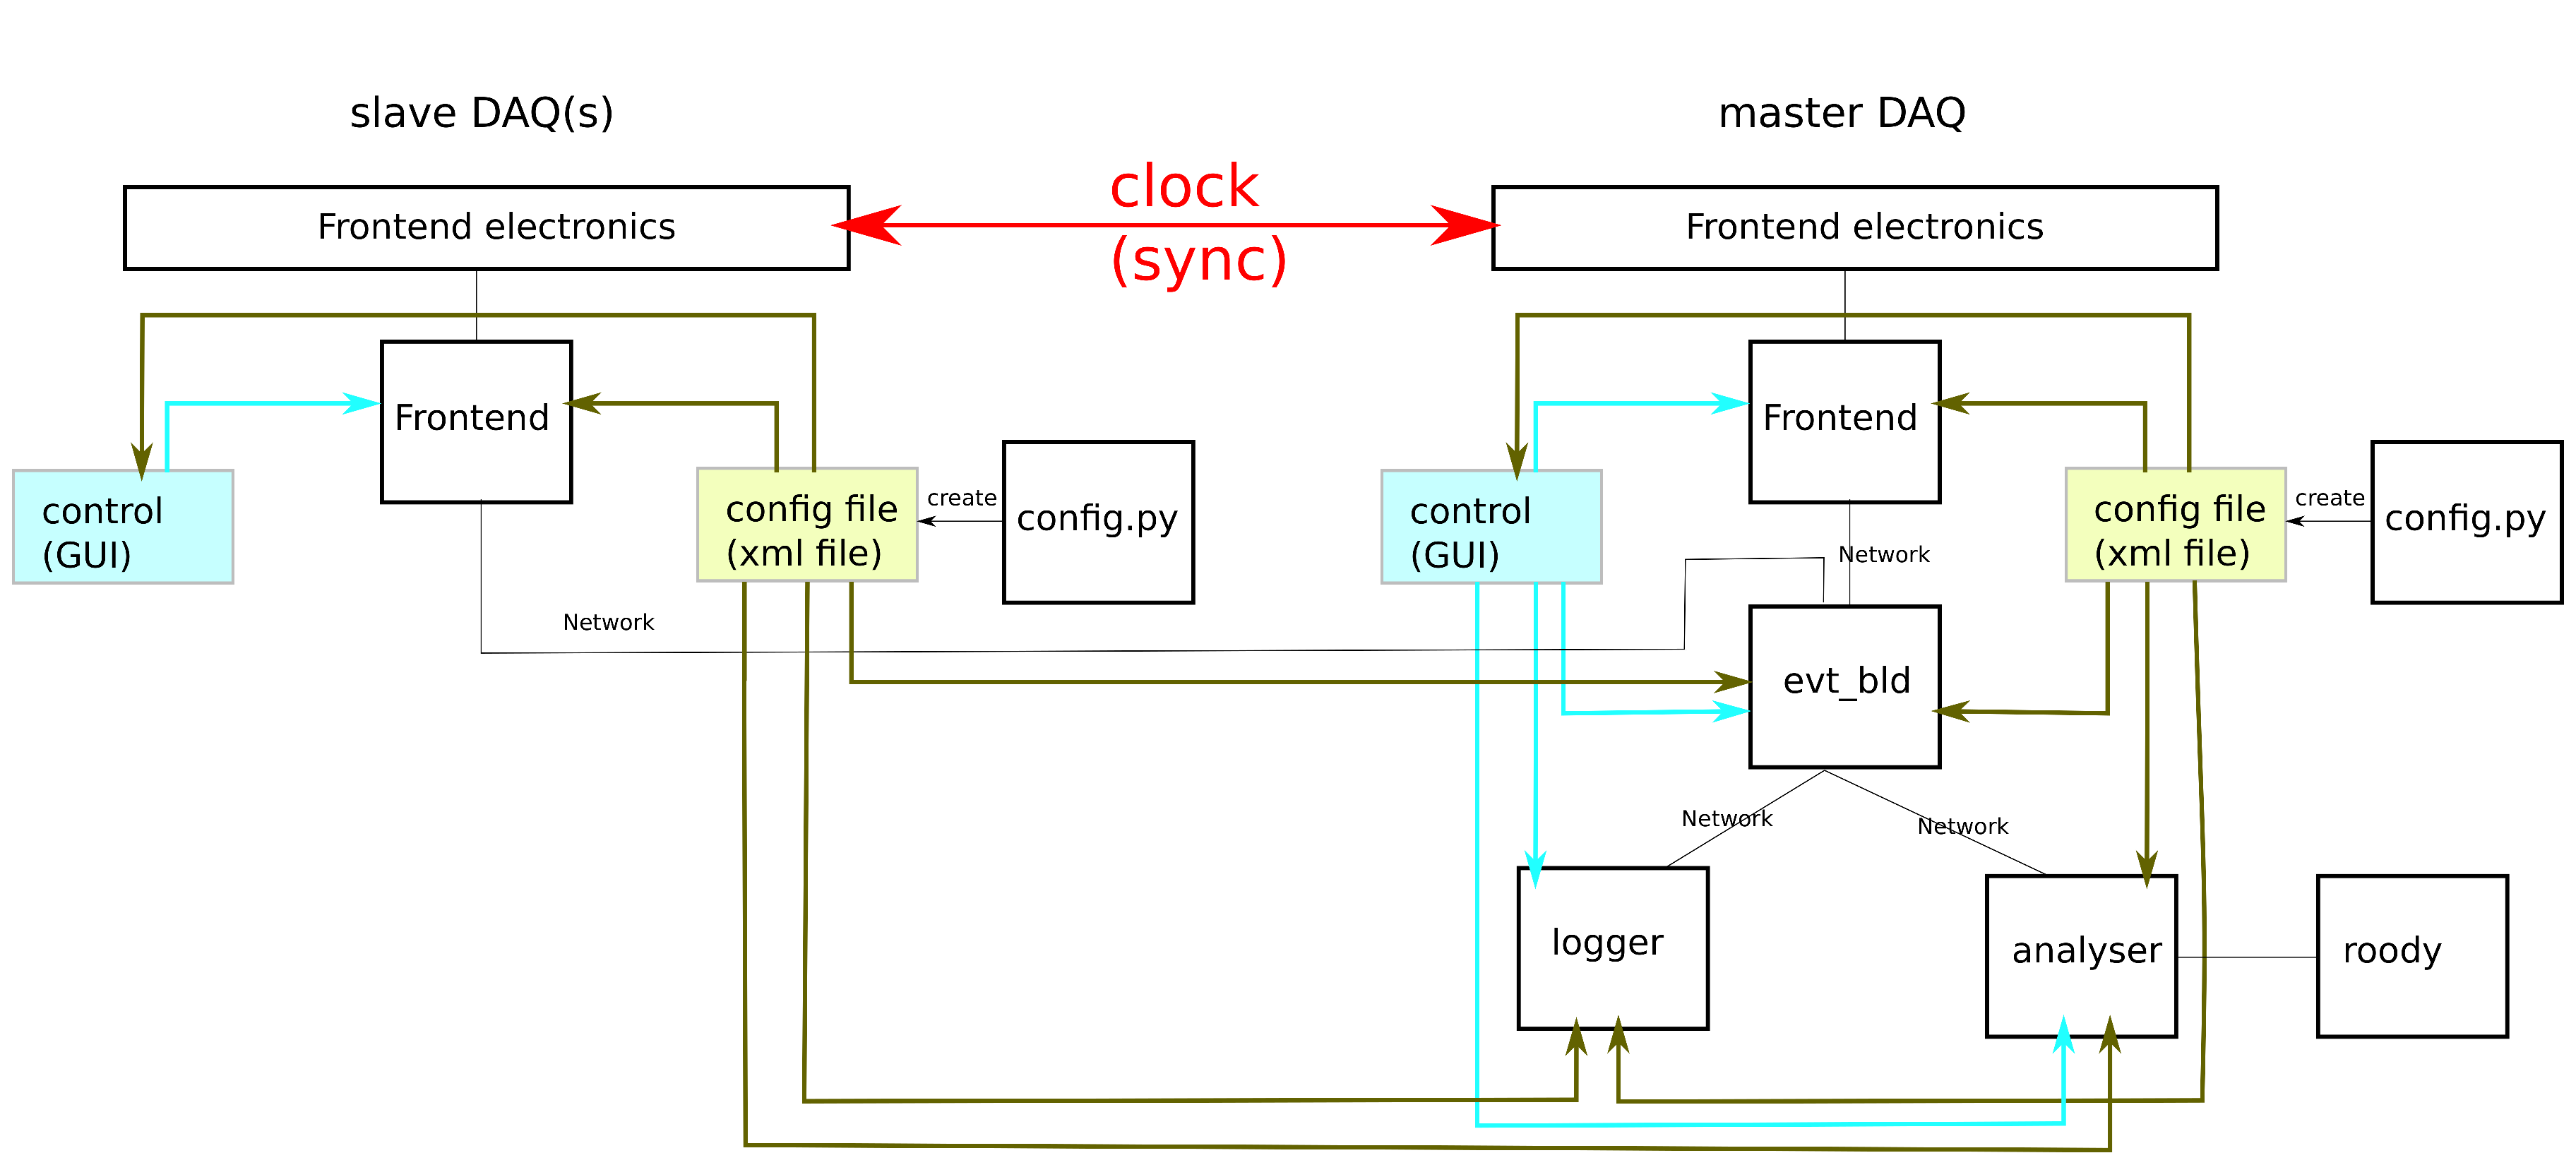
\includegraphics[width=.7\textwidth]{figs/daq_scheme2.eps}
			\caption{\label{fig02}Configuration of the DAQ with two DAQs}
		\end{center}
	\end{figure}
	When there are more than one DAQ needs to be used in an experiment, one
	can easily adjust the configuration as shown in Fig. \ref{fig02}. The
	only change is to change the evt\_bld to be connected with two frontends.

	\section{Frontend}
	To minimize the dead time of DAQ, the buffers of the modules should be
	utilized. However, this imposes the problem of synchronisation. To
	simplify the DAQ, it is required that all supported modules should have
	a time stamp for each event. This might be a strong limitation. If one
	really wants to use their modules which don't have time stamps, they
	should design their electronics such that for each event, a busy signal
	is issued, which is reset after reading the event. This basically means
	the buffers of the modules are disabled. So people are strongly advised
	to use modules with time stamps.  
	People may also need signals at the beginning and end of each run. 
	So one requirement is that 
	 \begin{tcolorbox}
	 after reading each event, a signal should be send out (for whatever purpose).
     At the beginning and end of each run, a signal should be send out. These
	 three signals should use different ports.
	 \end{tcolorbox}

	 To maximize the speed,
	 \begin{tcolorbox}
	 The same type of modules should be readout in BLT mode (if they are in
	 the same crate)
	 \end{tcolorbox}
	 For example, if one has five MADC32 (in the same crate), they should be
	 readout in BLT mode. Each BLT read may readout data for more than one
	 event, if they are all send out directly to the event builder without
	 preprocessing, the event builder will have to deal with a block of data
	 from multiple events from multiple modules.  It would be very difficult
	 for the event builder to build events based on their time stamps (in
	 principle it is still possible though). At the same time the
	 preprocessing done by the frontend should be kept minimum to keep it
	 fast enough. The final decision is like following:
	 \begin{tcolorbox}
		 In each BLT read, the data is packaged to contain the length of
		 data (in byte) and the id of module where the data is readout.
		 Then at the end of all readout, the whole data is packaged to
		 contain the total length,  the DAQ id, the offset of the first data
		 and the time stamp (from the operating system). Then the whole
		 package is send out to the event builder. See fig. \ref{fig03}.
	 \end{tcolorbox}
	 The time stamp from the operating system is helpful to let the event
	 builder determine the overflows of the time stamps of each module (see
	 the section on event builder). The offset of the first data is the
	 offset of the first fragment header within the whole data package. This
	 offset should be used to determine the beginning of data. It allows
	 variable length of the global header. The DAQ id may be useful if more
	 than 1 DAQs are present.
	 To maximize the speed, at multithread should be used in the
	 frontend: Two threads (one for trigger type and the other for scaler
	 type) read out data from modules and packs it, another sends
	 the data out to event builder via network. These threads use ring
	 buffer to shared data and sequence locks for synchronisation.
	 The structure of the ring buffer is shown in Fig. \ref{fig03}.
	 Another thread should be used to communicate with the GUI controller of
	 the DAQ. 





	\begin{figure}
		\begin{center}
			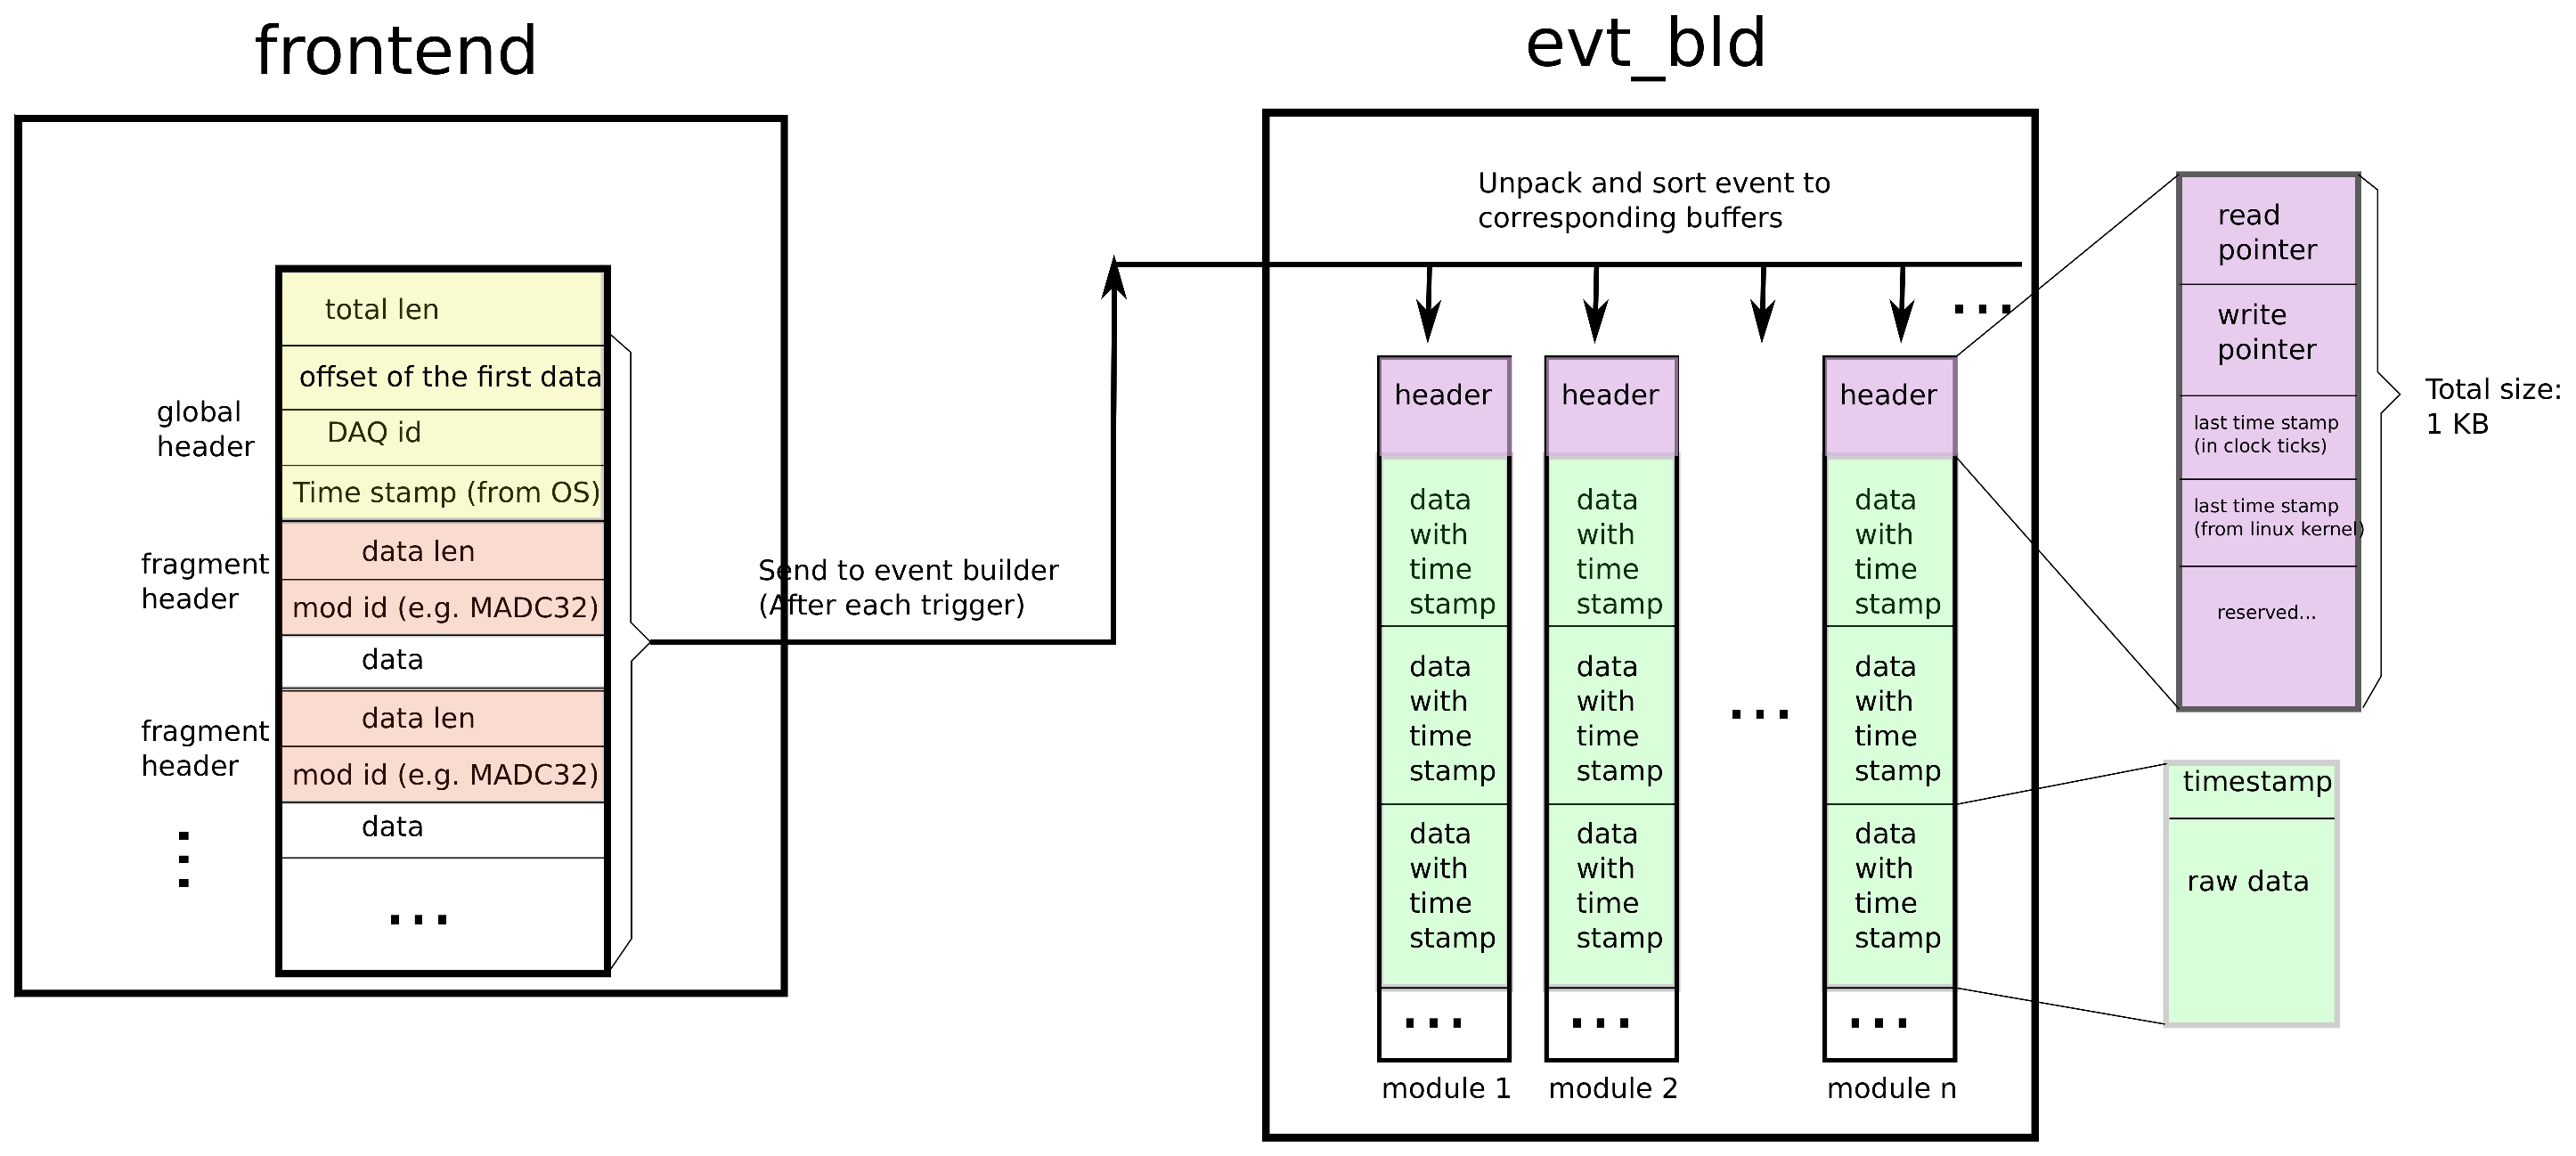
\includegraphics[width=.8\textwidth]{figs/data_format.eps}
			\caption{\label{fig03}Data structures in frontend and event
			builder. }
		\end{center}
	\end{figure}

	\section{event builder}
	The main task of event builder is to build event from the data send from
	frontend based on their time stamps. To make the building process
	easier, the following methods are employed:
	 \begin{tcolorbox}
		 After receiving each data package from frontend, the data are
		 sorted and saved to different buffers based on their origin. 
	 \end{tcolorbox}
	 Here each module has a buffer, not each type of module has a buffer.
	 For example, one has 5 MADC32, then 5 buffers are created, one for each
	 MADC. This is not too crazy. Imagine one has 100 modules for an
	 experiment, there are 100 buffers. However, each buffer doesn't have to
	 be very large. So the total memory consumption should not be a problem.
	 And this also makes the building event process easier.
	 \begin{tcolorbox}
		 In each buffer, the events should have been sorted based on their
		 time stamps.
	 \end{tcolorbox}
	 You can imagine this is also going to make the building process easier.
	 The time stamps at the beginning of each data blocks should be
	 monotonic (at least for each run). That means when sorting the events,
	 the event builder should be able to detect the overflows of time
	 stamps and correct for that. The header of each buffer has the value of
	 `the last time stamp' $T_{last}$ and `the last computer time'
	 $T^\prime_{last}$ to help to achieve
	 this. The $T_{last}$ is in unit of the clock ticks and the
	 $T^\prime_{last}$
	 is the time stamp added by the frontend (from linux kernel). The $T_{last}$
     is monotonic and never overflows. 
	 The
	 `computer time' added by frontend should also use the monotonic clock
	 provided by the kernel. 
	 From the $T_{last}$, it is straight forward to calculate the last
	 time stamp readout from module $t_{last}$ = ($T_{last}$ $ mod$ $ R$)
	 where $R$ is the range. For example, if one module has a time stamp of
	 40-bit length, the range is $R$ = 2$^{40}$.  Since each event has the
	 time stamp read out from module $t_{this}$ and time stamp added by
	 frontend $T^\prime_{this}$, we can use these information together with
	 those from the buffer header to get the following three quantities:
	 $\Delta T^\prime$, $t_{last}$ and $t_{this}$ which are the time interval
	 between the two events, last time stamp readout from module and the
	 current time stamp readout from module. These three quantities should
	 have enough information to let us determine the number of overflows
	 between the two events (if there are any).

	 How to build events?\\
	 Since each event in the buffers are already sorted by time, it is
	 straight forward to combine them into one events.
	 The tricky thing is when to start and stop to build
	 events? The most simple answer would be to start building events
	 immediately after receiving data from frontend and stop it when no more
	 data in the buffers. However, this approach may have some problems when
	 multiple events are readout in one data blocks. This is also shown in Fig.
	 \ref{fig04}. The data with time stamp $t4$ from module $m$ and module
	 $n$ should belong to one event, however, they won't be combined
	 together to form one event. A better way is to start building events
	 whenever received data from frontend, as before. However, we stop
	 building events as soon as any of the event buffers is empty. But there
	 is one exception: if the buffer is empty at the beginning of event
	 building, we should not stop. That means if we find out that one event
	 buffer is empty before we retrieve any data from it, it just means the
	 corresponding channel is not fired, we shouldn't stop our event
	 building process. To recap:
	 \begin{tcolorbox}
		 We start event building whenever we received data from frontend, we
		 stop event building if $any$ of the buffers is empty. However, if
		 one event buffer is already empty before we get any data out of it,
		 we won't stop event building even if this buffer is empty.
	 \end{tcolorbox}
	\begin{figure}
		\begin{center}
			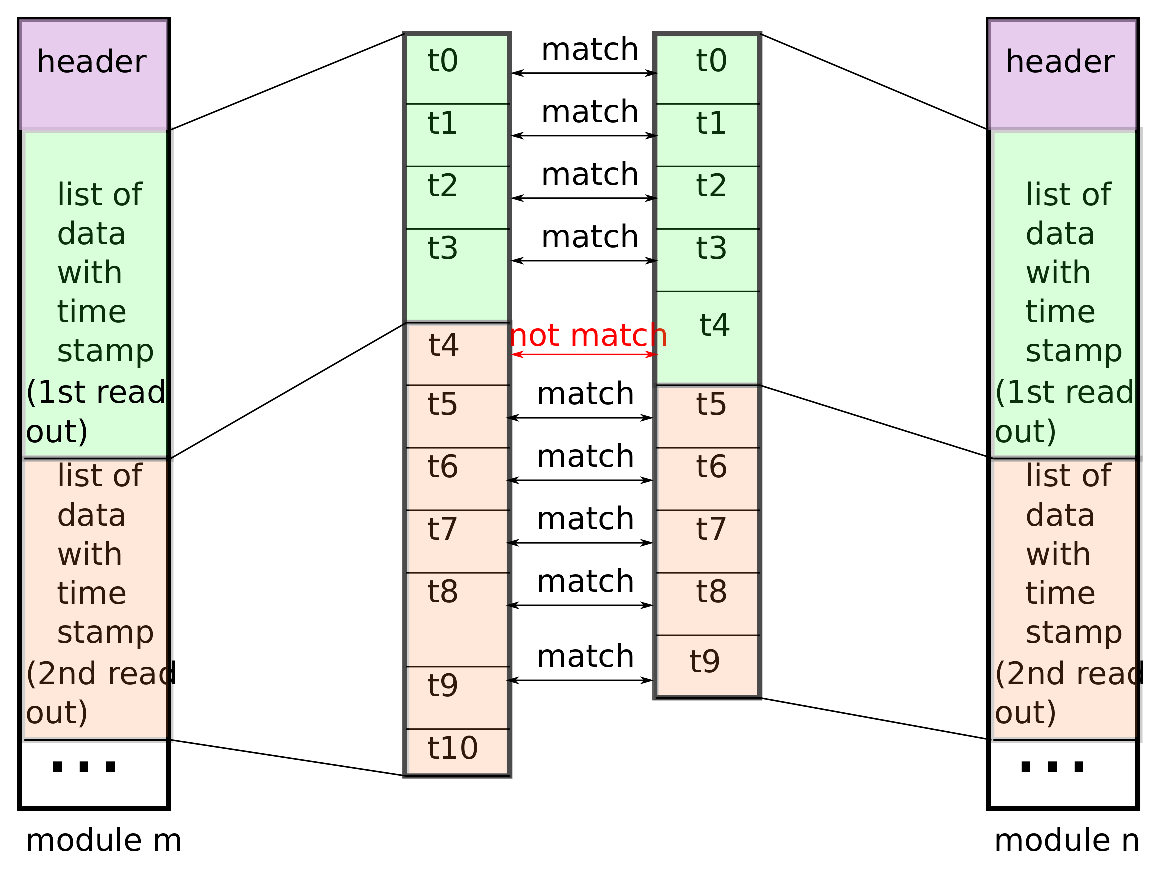
\includegraphics[width=.5\textwidth]{figs/combine_evt.eps}
			\caption{\label{fig04}Data structures in frontend and event
			builder. }
		\end{center}
	\end{figure}



	    




\end{document}
